% !TeX spellcheck = hu_HU
\documentclass[a4paper,12pt]{article}

% Magyar nyelvi beállítások
\usepackage[utf8]{inputenc}
\usepackage[T1]{fontenc}
\usepackage[magyar]{babel}

% Linkek
\usepackage[colorlinks, allcolors=blue]{hyperref}

% Szebb betűtípus
\usepackage{lmodern}

% Matematika
\usepackage{amsmath, amssymb, amsthm, amsfonts}

% Oldalmargók
\usepackage[margin=2.5cm]{geometry}

% Színes dobozok definíciókhoz, tételekhez stb.
\usepackage{tcolorbox}
\tcbuselibrary{theorems}

%coordinate
\usepackage{tikz}

% Tételstílusok
%no counter / number within=section
\newtcbtheorem[no counter]{definition}{Def.}%
{colback=blue!5,colframe=blue!50!black,fonttitle=\bfseries}{def}

\newtcbtheorem[no counter]{theorem}{Tétel}%
{colback=green!5,colframe=green!50!black,fonttitle=\bfseries}{th}

\newtcbtheorem[no counter]{example}{Példa}%
{colback=yellow!10,colframe=yellow!50!black,fonttitle=\bfseries}{ex}

\newtcbtheorem[no counter]{remark}{Megjegyzés}%
{colback=gray!10,colframe=gray!50!black,fonttitle=\bfseries}{rem}

\newtcbtheorem[no counter]{observation}{Megfigyelés}%
{colback=orange!5, colframe=orange!80!black, fonttitle=\bfseries}{obs}

\newtcbtheorem[no counter]{statement}{Allítás}%
{colback=orange!5, colframe=red!80!black, fonttitle=\bfseries}{sta}

% Fejezetcímekhez kicsit szebb stílus
\usepackage{titlesec}
\titleformat{\section}{\Large\bfseries}{\thesection.}{0.5em}{}
\titleformat{\subsection}{\large\bfseries}{\thesubsection.}{0.5em}{}

\begin{document}

\title{Algoritmikus játékelmélet}
\author{Ács Dorottya, Gutbrod Ádám}
\date{2025}
\maketitle

\tableofcontents
\newpage



%Kombinatorikus játék fogalma, éles játék, betli játék, nyerő stratégia. Irányított gráf magja, mag egyértelműsége DAG-ban. Játékok, ill. pozíciók típusa.
\section{Tétel}
\begin{definition}{Kombinatorikus játék}{}
$ J=(G,N_W,N_L,N_T,V_0) $, ahol $ G DAG, N_W,N_L,N_T$ nyelők partíciója és $v_0 \in V(G)$ kiinduló állapot
\end{definition}
Tulajdonságai:
\begin{itemize}
    \item Kétszemélyes és szekvenciális: a két játékos felváltva lép
    \item A játéknak kétféle kimenetele van: vagy az egyik játékos nyer és a másik veszt, vagy pedig döntetlen.
\end{itemize}
Példák:
\begin{itemize}
    \item Mérgezett csoki
    \item Sakk
    \item Nim
\end{itemize}

\begin{definition}{Éles játék}{}
Éles játék: $N_L \cup N_T=\varnothing$
\end{definition}

\begin{definition}{Betli játék}{}
Betli játék: $N_W \cup N_T = \varnothing$
\end{definition}

\begin{observation}{}{}
Ha $N_T = \varnothing \Rightarrow \forall$ kombinatorikai játék v.vhető éles játékra.
\end{observation}

Biz.: Bevezetünk egy extra csúcsot és $\forall N_L$-beli csúcsból 1-l ir. élt ide \\
\begin{theorem}{Gráf csúcsok típusa}{}
    Tetszőleges éles kombinatorikus játékban $\forall$ csúcshoz egyértelműen eldönthető, hogy I vagy II típusú.
\end{theorem}

\begin{itemize}
    \item I-es típusú csúcsból indulva a kezdő garantálni tudja a győzelmet
    \item II-es típusú csúcsból indulva a másodiknak lépő játékos tudja garantálni azt
\end{itemize}

Biz.: Fordított topologikus sorrendben meghatározzuk $\forall$ csúcs típusát,
$v_i típusa$ ...
\begin{itemize}
    \item II-es típusú, ha $\nexists v_iv_j \in E(G)$, amire $v_j$ típusa II-es
    \item  I-es, ha $\exists v_iv_j \in E(G)$, amire $v_j$ II-es\\
    (És ez a két eset egymás komplementere.)
\end{itemize}


\begin{observation}{}{}
    II-es típusú csúcsok halmaza:
    \begin{itemize}
        \item független 
        \item $\forall$ nem II-esből vezet él II-esbe
    \end{itemize}
\end{observation}

\begin{definition}{Stratégia}{}
    Stratégia alatt egy V → V függvényt értünk, amely minden V -beli helyzethez amelyik nem nyelő, hozzárendeli az egyik ki-szomszédját: vagyis tetszőleges álláshoz hozzárendelünk egyet a lehetséges lépések közül. Egy játékos követi az adott stratégiát, ha mindig a stratégia által kijelölt pozícióba lép. 
\end{definition}

\begin{definition}{Nyerő stratégia}{}
    Nyerő egy stratégia, ha őt követve mindig nyerni tudunk, akármit is lépjen közben a másik játékos.
\end{definition}

\begin{definition}{Mag}{}
    G irányított gráf magja a csúcsok olyan független M részhalmaza, amikbe $\forall$ M-en kívüli csúcsból vezet él.
\end{definition}
Köv.: G DAG $\Rightarrow$ G-ben $\nexists$ mag

\begin{definition}{Játék típusa}{}
    A $J = (v, N_W, v_0)$ éles játék típusa $v_0$.
\end{definition}



\newpage
%Játékok összege, az összeg típusa. Grundy-számozás. NIM-összeadás és tulajdonságai.
\section{Tétel}
\begin{definition}{Játékok összege}{}
    A $J_1 + J_2$ játék kimenetelét az utolsónak befejezett játék határozza meg.
\end{definition}

\begin{definition}{Grundy-számozás}{}
    G ir. gráfnak $g: V(G) \rightarrow \mathbb{N}$ Grundy-számozása, ha $g(v)=mex \{g(n): vu\in E(G)\}$ 
\end{definition}

\begin{observation}{}{}
	\begin{itemize}
		\item $J + J\rightarrow$ II-es típusú (másolás)
		\item $II_1 + II_2\rightarrow$ II-es típusú (mindkettőt meg tudja nyerni a 2. játékos)
		\item $I + II\rightarrow$ I-es típusú (a kezdő az I-es játékban a nyerő stratégiája szerint lép)
		\item $I + I\rightarrow$ nem egyértelmű...
	\end{itemize}
\end{observation}

\begin{statement}{}{}
	$G$ véges DAG $\Rightarrow G$-nek $\exists$! Grundy-számozása.
\end{statement}
Biz: $\exists$ topológikus sorrend, ebben visszafelé haladva egyértelműen adódik minden csúcsé.
	
\begin{statement}{}{}
	Tfh. $J_1$ kezdőállapotának Grundy-száma $g_1, J_2$ kezdőállapotáé $g_2$. \\
	$J_1 + J_2$ típusa I-es, ha $g_1 \not= g_2$, és II-es ha $g_1 = g_2$.
\end{statement}
Biz: 
\begin{itemize}
	\item Tfh. $g_1=g_2$. \\
	Ekkor a 2. játékos nyerni tud azzal, hogy mindigy úgy lép, hogy a két állapot Grundy-száma megegyezzen.
	\item Tfh. $g_1 \not= g_2$.  \\
	Ekkor a kezdő nyer azzal, hogy a nagyobbik g-t a kisebbikre csökkenti.
\end{itemize}

		
\begin{theorem}{}{}
    $g(v_1v_2) = g_1(v_1)\oplus g_2(v_2)$
\end{theorem}

\begin{definition}{NIM-összeadás (bitenkénti XOR)}{}
    $a \oplus b = c$ a NIM-összeadás, ahol $c$-t úgy kapjuk, hogy $a$ és $b$ 2-es számrendszerbeli alakját írásban összeadjuk, de a maradékot elfelejtjük. 
\end{definition}

\begin{observation}{NIM-összeadás tulajdonságai}{}
    \begin{itemize}
        \item $a\oplus b = b\oplus a$
        \item $(a \oplus b ) \oplus c = a \oplus (b \oplus c)$
        \item $a \oplus a = 0$
        \item $a \oplus b = a \oplus b'\Rightarrow b=b'$
        \item $c < a \oplus b \Rightarrow \exists a' < a: c =a' \oplus b$ vagy $\exists b' < b: c =a \oplus b'$
    \end{itemize}
\end{observation}
Biz: \\

\newpage
%Sprague–Grundy-tétel, Bouton-tétel. Játékok izomorfiája és ekvivalenciája
\section{Tétel}
\begin{theorem}{Sprague–Grundy}{}
	 Ha u és v $J_1 és J_2$ kombinatorikus játékokban állások, akkor $g_{J_1,J_2}(u, v) = g_{J_1}(u) \oplus g_{J_2}(v)$
\end{theorem}

\begin{theorem}{Bouton}{}
	k-nim II-es típusú $\Leftrightarrow n_1 \oplus n_2 \oplus ... \oplus n_k = 0$, ahol $nn_1, ... n_k$ a kupacok méretei.
\end{theorem}

\begin{definition}{Játékok izomorfia}{}
	$J = (G, N_W, N_T, N_L, v_0)$ kombinatorikus játék izomorf $J' = (G', N_W', N_T', N_L', v_0')$ kombinatorikus játékkal, ha van olyan $G \cong G'$ gráfizomorfia, hogy $N_W$ és $N_W'$, $N_T$ és $N_T'$, $N_L$ és $N_L'$, $v_0$ és $v_0'$ egymásnak felelnek meg.
\end{definition}

\begin{definition}{Ekvivalencia}{}
	$J_1$ és $J_2$ kombinatorikus játék $u_0$ és $v_0$ kezdőpozíciókkal ekvivalensek, ha...
	\begin{itemize}
		\item $J_1 + J_2 = II$
		\item $g_{J_1}(u_0) = g_{J_2}(v_0)$
		\item $\forall H$ kombinatorikus játékban igaz $H + J_1$ és $H + J_2$ azonos típusúak
	\end{itemize}
\end{definition}

\newpage
\section{Tétel}
\begin{definition}{Stratégia lopás}{}
	Bizonyítási módszer arra, hogy...
	\begin{itemize}
		\item ha nincs döntetlen, akkor az első játékosnak van nyerő stratégiája
		\item ha van döntetlen, akkor az elsőnek van nem vesztő
	\end{itemize}
\end{definition}

\begin{theorem}{Mérgezett csoki / Chomp}{}
	A kezdőjátékosnak van nyerő stratégiája
\end{theorem}

Biz.: nincs döntetlen\\
Tegyük fel indirekt: a második játékosnak van nyerő stratégiája. Ekkor van jó válasza arra, ha a kezdő a jobb felső (n, m) kockát eszi meg. Legyen az (i, j). Lépjük ezt az (i, j) kockát első játékosként. Ezután játssza az első játékos az eredeti második nyerő stratégiája szerint.

\begin{theorem}{Hex}{}
	Az első játékosnak van nyerő stratégiája
\end{theorem}

Biz.: nincs döntetlen + stratégialopás \\
Vegyük a künöböző színű mezők közötti mezőhatárokat. Írjunk ezekbe irányított éleket. \\
Bal felső nagy nyílból kiindulva lépek az élek mentén, elakadni nem fogok, önmagába visszafordulni se, mert nem létezhet 3 irányított éllel szomszédos pont, tehát valamelyik nagy nyílba fogok elérkezni. Ekkor a kapott útnak egyik oldalon csupa azonos színű, a megfigyelt 2 térfélt összekötő utat kapunk.\\
\begin{center}
	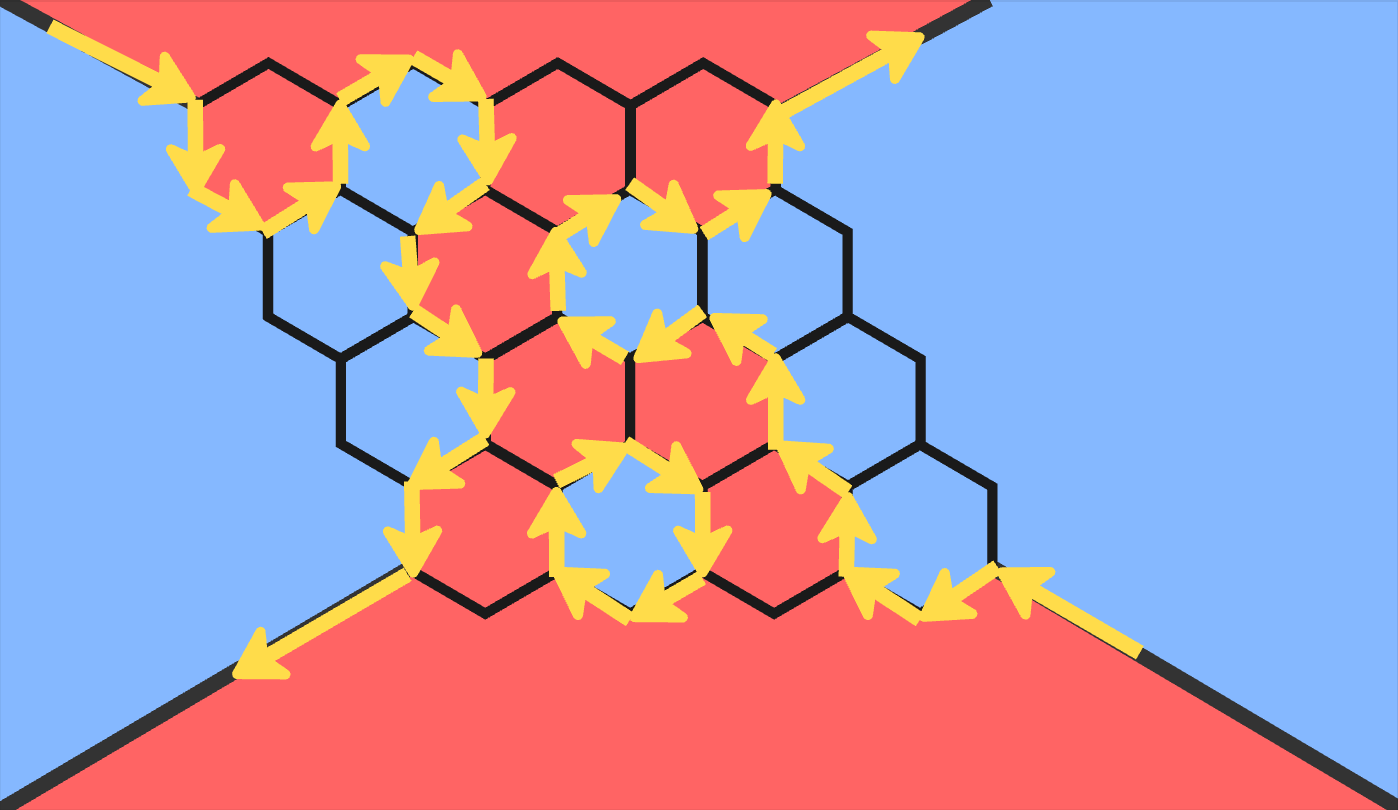
\includegraphics[width=90mm]{hex_biz}
\end{center}


\begin{theorem}{Véges amőba}{}
	Az elsőnek van nem vesztő stratégiája
\end{theorem}
Biz.: indirekten tegyük fel, hogy a második játékosnak van nem vesztő stratégiája \\
Első játékos: X, második játékos: O\\
Játsszon az első játékos egy olyan táblán, amire ő gondolatban valamilyen (i, j) mezőre egy X-et odaképzelt. Játssza ezen a képzeletbeli táblán az első játékos a második játékos nyerő stratégiáját. Ha a második pont erre az (i, j) mezőre tesz, akkor válasszon az első egy tetszőleges másik üres mezőt és képzelje oda az X-et $\rightarrowtail$ (i', j'). \\
A játék végén: a képzelt táblán az első nem fog veszíteni, tehát a valódin sem.

\newpage
\section{Tétel}
\begin{definition}{Stratégiai játékok}{}
	n játékos van $1\leq i \leq n$ esetén $S_i$ az i-edik játékos lehetséges stratégiája $S = S_1 \times S_2 \times ...  \times S_n$ stratégiaválasztások (kimenetelek) halmaza.\\
	$u_i : S \longrightarrow \mathbb{R}$ i-edik játékos nyereség függvénye.
\end{definition}

$\forall$ stratégiai játékra teljesül
\begin{itemize}
	\item 1 lépéses, szinkron
	\item teljes információs ($\forall$ játékos tisztában van  $\forall$ másik játékos stratégiájával)
	\item $\forall$ játékos racionális ($\forall$ játékos a nyereségét akarja maximalizálni)
\end{itemize}

További lehetséges tulajdonságok
\begin{itemize}
	\item 0-összegű, ha $\sum_{i=1}^{n}{}u_i(s) = 0$  $\forall \quad s \in S$ (egy stratégiai választás)
	\item szimmetrikus, ha $\exists k$, amire $|S_i|= k$ és ezek a stratégiák megszámlálhatók úgy 1-től k-ig, hogy $\forall \pi$ permutációra [n-en] $\forall 1\leq i \leq n \quad v_i(s)=u_{\pi (i)}(s_{\pi}) \quad \forall s \in S$
\end{itemize}

\begin{center}
\begin{tabular}{llll}
	\hline
	\multicolumn{1}{|l|}{}  & \multicolumn{1}{l|}{K}     & \multicolumn{1}{l|}{P}     & \multicolumn{1}{l|}{O}     \\ \hline
	\multicolumn{1}{|l|}{K} & \multicolumn{1}{l|}{0, 0}  & \multicolumn{1}{l|}{-1, 1} & \multicolumn{1}{l|}{1, -1} \\ \hline
	\multicolumn{1}{|l|}{P} & \multicolumn{1}{l|}{1, -1} & \multicolumn{1}{l|}{0, 0}  & \multicolumn{1}{l|}{-1, 1} \\ \hline
	\multicolumn{1}{|l|}{O} & \multicolumn{1}{l|}{-1, 1} & \multicolumn{1}{l|}{1, -1} & \multicolumn{1}{l|}{0, 0}  \\ \hline
	\multicolumn{4}{l}{Kő-papír-olló strat. mátrix}                                                               
\end{tabular}
\end{center}
	


\begin{definition}{Fogolydilemma}{}
	content...
\end{definition}

\begin{center}
	\begin{tabular}{lll}
		\hline
		\multicolumn{1}{|l|}{}     & \multicolumn{1}{l|}{önző}              & \multicolumn{1}{l|}{koop}         \\ \hline
		\multicolumn{1}{|l|}{önző} & \multicolumn{1}{l|}{-100 + e, -100 +e} & \multicolumn{1}{l|}{-1 + e, -100} \\ \hline
		\multicolumn{1}{|l|}{P}    & \multicolumn{1}{l|}{-100, -1 + e}      & \multicolumn{1}{l|}{-1, -1}       \\ \hline
		\multicolumn{3}{l}{Fogoly-dilemma}                                                                     
	\end{tabular}
\end{center}

\begin{definition}{Százlábú játék}{}
	nem tudom, hogy ez kell-e
\end{definition}

\begin{definition}{Iterált szigorú eliminálás}{}
	A dominált stratégiát töröljük, és ezt a lépést domináljuk
\end{definition}

\begin{definition}{Iterált laza eliminálás}{}
	Ha gyengén dominált stratégiát törlünk.
\end{definition}

\begin{theorem}{Ennek mi a neve?}{}
	Iterált szigorú eliminálásokat végezve, amíg lehet, mindig ugyanazt a játékot kapjuk
\end{theorem}
Biz.:\\
Tfh.: $s_1, s_2, ... s_l$ sorrendben szigorúan eliminálva további elimináció nem végezhető, ill. $z_1, z_2, ... z_t$ stratégiákra ugyanezt. Cél $\{ s_1, s_2, ... s_l\} = \{z_1, ... z_t\}$\\
Indirekt: Tfh. $\neq$, azaz  $\exists s_i \notin \{z_1, ... z_t\}$\\
Legyen $i$ min erre!\\
$s_1, s_2, ... s_{i-1} \in \{z_1, z_2 ... z_t\} \Longrightarrow z$ eliminálása után $s_i$ dominált.

\begin{definition}{Pareto-optimális stratégiaválasztás}{}
	$s, s' \in S, \quad s \quad$Pareto-dominálja s'-t, ha $u_i(s) \geq u_i(s') \quad \forall i \in [n]$ és $\exists j \in [n] : u_j(s) > u_j(s')$\\
	$s \in S$ strat. választás Pareto-optimális, ha semelyik más strat. választás sem Pareto-dominálja
\end{definition}

[csinálok ide ábrát]

\newpage
\section{Tétel}
\begin{definition}{Nash-egyensúly (NE)}{}
	$s \in S$ tiszta Nash-egyensúly, ha egyetlen játékosnak sem érdeke más stratégiát választani azaz $u_i(s) \geq u_i(s',s_{-i}) \quad \forall \; 1 \leq i \leq n \quad \forall s' \in S$
\end{definition}
Példa: fogoly-dillemmában van ilyen, kő-papír-ollóban nincs

\begin{theorem}{(iterált) eliminálás
		hatása a Nash-egyensúlyokra}{}
	Szig. elim. hatására a tiszta NE-k (tNE) halmaza nem változik
\end{theorem}
Biz.: \\
Tfh.: $s \in S_i$ dominálja $s' \in S_i$-t és $s'$-t töröljük

\begin{observation}{}{}
	Törlés előtt tNE nem tartalmazta s'-t 
\end{observation}
Következmény: $\forall$ törlés tNE a törlés után is tNE marad \\
Tfh.: z tNE a törlés után. Ha z nem tNE a törlés előtt $u_i(s', z_{-i}) > u_i(z)$

\newpage
\section{Tétel}
\begin{definition}{Kevert stratégia}{}
	$\sigma : s_i \rightarrow \mathbb{R}_+$ kevert stratégia, ha $\sum_{s_i \in S_i} \sigma_i(s_i) = 1$ \\
	$\Delta_i$: ezek halmaza $\rightarrow$ i-dik játékos kevert stratégiái 
	$s_i \in S_i$-hez tartozó tiszta stratégia \\
	$\chi_{s_i}$-vel jelöljük: 
	\[
	\chi_{s_i}(s') =
	\begin{cases}
		1 & \text{if } s' = s_i, \\
		0 & \text{if } s' \neq s_i
	\end{cases}
	\] 
	$\Delta = \Delta_1 \times , ..., \times \Delta_n$: kevert stratégia választások halmaza \\
	$\sigma \in \Delta$ (kevert strat. választás), \quad $s \in S$ (konkrét strat. választás) ($\rightarrow$ rögzítünk egy konkrét strat. választást) $P_\sigma (s) = \prod_{i=1}^n \sigma_i(s_i) $ (független események)\\
	$\sigma = (\sigma_1, ..., \sigma_n) \quad s=(s_1, ..., s_n) \quad u_i(\sigma) = \sum_{s \in S} P_\sigma (s) \cdot u_i(s)$ i-dik  játékos nyeresége, várható nyereség
\end{definition}

\begin{definition}{Legjobb válasz}{}
	$s_{-i} = (s_1, ..., s_n) \in S_{-i},$ (i-dik játékos kivételével mindenkinek választottunk stratégiát) esetén $s_i$ az i-dik játékos számára legjobb válasza, ha $u_i(s_i,s{-i}) \geq u_i(s_i',s_{-i}) \quad \forall s_i \in S$
\end{definition}

Láttuk: $s \in S$ tNE, ha $\forall$ i-re $s_i$ legjobb válasza $s_i$-re, ahol $s = (s_1, ..., s_n)$

\begin{definition}{Legjobb kevert stratégia}{}
	$\sigma_{-i} \in \Delta_{-i}$ esetén $s_i \in S$ az i-dik játékos számára legjobb tiszta stratégiai választás, ha $u_i(s_i \sigma_{-i}) \geq u_i(s_i'\sigma_{-i}) \quad \forall s_i' \in S_i$-re
\end{definition}

$\sigma_i$ az i-dik játékos számára legjobb kevert stratégia, ha $u_i(\sigma_i, \sigma_{-i}) \geq u_i(\sigma_i', \sigma_{-i})$

\begin{observation}{Legjobb tiszta válasz}{}
	$\sigma_i$ az i-dik játékos számára legjobb kevert strat. $\Leftrightarrow \quad \sigma_i = \sum_{s \in S_i} \lambda_s \chi_s$, ahol $\lambda_s > 0$ esetén s legjobb tiszta válasz
\end{observation}

Biz.: [...]

\begin{definition}{}{}
	$\sigma = (\sigma_1, ..., \sigma_n) \in \Delta$ kevert Nash-egyensúly, ha $\sigma_i$ legjobb kevert k strat $\sigma_{-i}$-re $\forall 1\leq i \leq n$
\end{definition}

Pl.: kó-papír-olló
\begin{center}
	\begin{tabular}{llll}
		\hline
		\multicolumn{1}{|l|}{}  & \multicolumn{1}{l|}{K}     & \multicolumn{1}{l|}{P}     & \multicolumn{1}{l|}{O}     \\ \hline
		\multicolumn{1}{|l|}{K} & \multicolumn{1}{l|}{0, 0}  & \multicolumn{1}{l|}{-1, 1} & \multicolumn{1}{l|}{1, -1} \\ \hline
		\multicolumn{1}{|l|}{P} & \multicolumn{1}{l|}{1, -1} & \multicolumn{1}{l|}{0, 0}  & \multicolumn{1}{l|}{-1, 1} \\ \hline
		\multicolumn{1}{|l|}{O} & \multicolumn{1}{l|}{-1, 1} & \multicolumn{1}{l|}{1, -1} & \multicolumn{1}{l|}{0, 0}  \\ \hline
		\multicolumn{4}{l}{Kő-papír-olló strat. mátrix}                                                               
	\end{tabular}
\end{center}

$\sigma_1 = (1/3, 1/3, 1/3) \quad \sigma_2 = (1/3, 1/3, 1/3)$

\[
legjobb tiszta válaszok
\begin{cases}
	u_1(k, \sigma_2) = 1/3(0+1-1)=0 \\
	u_1(k, \sigma_2) = 1/3(1+0-1)=0 \\
	u_1(k, \sigma_2) = 1/3(-1+1+0)=0
\end{cases}
\]

\begin{theorem}{}{}
	$\forall$ strat játéknak van kevert Nash-egyensúlya
\end{theorem}

Nem bizonyítjuk

\begin{definition}{}{}
	$\sigma_i \in \Delta_i$ erősen dominálja az $s \in S_i$ stratégiát, ha $u_i(\sigma_i, \sigma_{-i}) > u_i(s, \sigma_{-i}) \quad \forall \sigma_{-i} \in \Delta_{-i}$
\end{definition}

\begin{definition}{}{}
	$\sigma_i \in \Delta_i$ gyengén dominálja az $s \in S_i$ stratégiát, ha $u_i(\sigma_i, \sigma_{-i}) \geq u_i(s, \sigma_{-i}) \quad \forall \sigma_{-i} \in \Delta_{-i}$
\end{definition}

[példa ábra]

\begin{definition}{Szigorú / laza eliminálás}{}
	erősen / gyengén dominált strat. törlése
\end{definition}

\begin{definition}{}{}
	Iterált szig. / laza elim. ...
\end{definition}

\begin{statement}{}{}
	Szig. elim.-sal kNE nem tűnik el
\end{statement}

Biz.: [...]

\begin{statement}{}{}
	Laza. elim. után kapott kNE az elim. előtti játékba is kNE
\end{statement}

Biz.: [...]

\newpage
\section{Tematika}
\begin{enumerate}
	\item Kombinatorikus játék fogalma, éles játék, betli játék, nyerő stratégia. Irányított gráf magja, mag
	egyértelműsége DAG-ban. Játékok, ill. pozíciók típusa.
	\item Játékok összege, az összeg típusa. Grundy-számozás. NIM-összeadás és tulajdonságai.
	\item Sprague–Grundy-tétel
	, Bouton-tétel. Játékok izomorfiája és ekvivalenciája.
	\item Stratégialopás. Mérgezett csoki, amőba, hex.
\end{enumerate}

\newpage
\section{Források}
\begin{itemize}
    \item Dr. Fleiner Tamás és Nemkin Viktória előadásán elhangzottak
    \item Algoritmikus játékelmélet szóbeli tematika 2024 \url{https://www.cs.bme.hu/\%7Efleiner/alje2024/tematika.pdf}
    \item Végh László, Király Tamás, Pap Júlia: Játékelmélet jegyzet \url{http://tkiraly.web.elte.hu/students/jatekelmelet_jegyzet.pdf}
    \item Bernhard von Stengel: Game Theory Basics \url{http://www.maths.lse.ac.uk/personal/stengel/lectnotes1-7.pdf}     
\end{itemize}

\end{document}
